\subsection{Amplificador de Instrumentación}

\subsubsection{Introducción}

Un \textbf{amplificador diferencial} es un dispositivo electrónico como el visto en la FIGURA que amplifica la diferencia de sus señales de entrada. Idealmente, su configuración resulta tal que amplifica únicamente señales en \textbf{modo diferencial} mientras que rechaza por completo señales en \textbf{modo común}, definiéndose éstas como:

$$V_{DM}=V_{2}-V_{1}$$

$$V_{CM}=\frac{V_{1}+V_{2}}{2}$$

A partir de esto, se definen la \textbf{ganancia en modo común} y la \textbf{ganancia en modo diferencial}, respectivamente, de la siguiente forma:

$$A_{CM} = \frac{V_{out_{CM}}}{V_{CM}}$$

$$A_{DM} = \frac{V_{out_{DM}}}{V_{DM}}$$

La Razón de Rechazo en Modo Común (CMMR, por sus siglas en inglés) es un parámetro que indica el rechazo que ofrece el circuito a una entrada en modo común y es definido en decibelios por la relación entre la ganancia en modo diferencial y la ganancia en modo común. 

$$CMRR_{dB} = 20\cdot \log_{10}\left | \frac{A_{DM}}{A_{CM}} \right |$$

Un amplificador diferencial ideal posee una ganancia en modo diferencial tendiente a infinito y una ganancia en modo común igual a cero, ya que rechaza por completo las señales que ingresan con igual tensión por ambas entradas del operacional. Esta característica se logra con la correcta disposición y balance entre resistencias del circuito. En particular, en la FIGURA se logrará un completo rechazo a las señales en modo común cuando se cumpla la llamada condición de puente balanceado:

$$R_1\cdot R_4 = R_2\cdot  R_3$$

Dado que todos los componentes pasivos cuentan con una cierta tolerancia de fabricación, resulta difícil cumplir esta condición y, por lo tanto, conseguir un CMRR tendiente a infinito. 

Un \textbf{amplificador de instrumentación} (In Amp) es un dispositivo que actúa como un amplificador diferencial de precisión, ya que permite amplificar señales diferenciales de baja amplitud y elimina el ruido común a ambas entradas. Los In Amp de tres operacionales parten de una configuración circuital básica que consta de una etapa de entrada no inversora simétrica, la cual contribuye a lograr una alta impedancia de entrada y amplifica las señales de modo diferencial, y una etapa de salida diferencial. Su ganancia en modo diferencial puede ser modificada cambiando el valor de la impedancia $R_G$ entre los dos operacionales de entrada. Los $In$ $Amp$ se caracterizan por tener una alta impedancia de entrada (idealmente infinita); impedancia de salida baja (idealmente cero); ganancia estable y un CMRR alto (normalmente del orden de los 100dB). Por las características descriptas, estos amplificadores son utilizados en aplicaciones de precisión como ser sistemas de control, instrumentación médica, sistemas de audio, entre otras. 

En esta sección del presente trabajo se analizarán el comportamiento y características de un amplificador de instrumentación. Se partirá de un análisis matemático del circuito para obtener parámetros relevantes para luego realizar mediciones sobre el circuito y poder así contrastar con los modelos teóricos y los resultados simulados. 

\subsection{Descripción del comportamiento del circuito}

Con lo descripto en la introducción, realizará un análisis del comportamiento del siguiente circuito:

\begin{figure}[H]
    \centering
    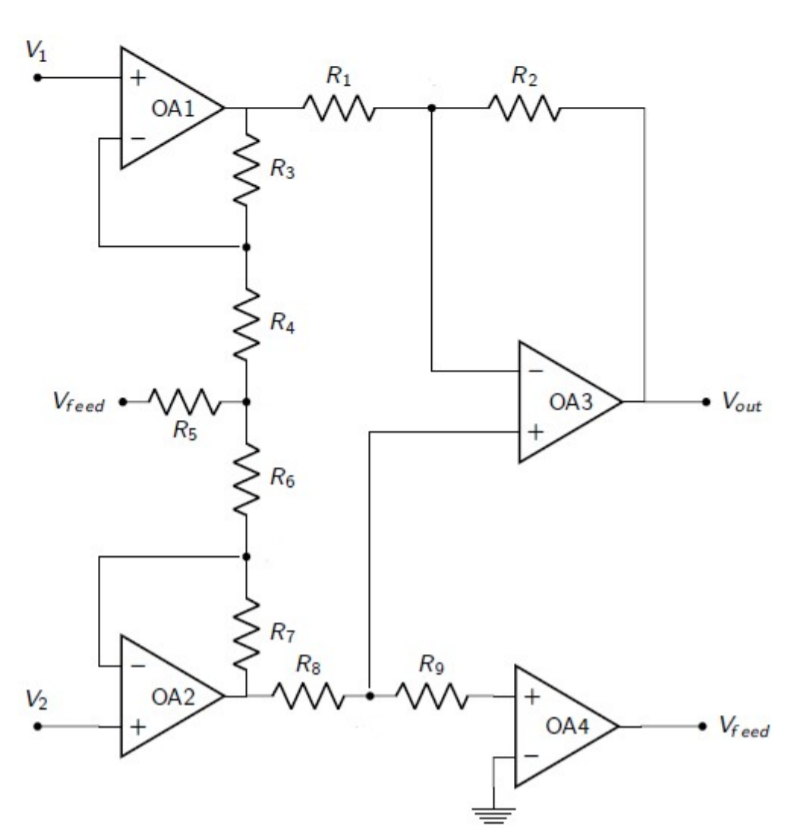
\includegraphics[scale=0.8]{../Ejercicio3-AmplificadorDeInstrumentacion/Imagenes/InAmpWiki.png}
    \caption{Señal de entrada cuadrada y salida del circuito RLC}
    \label{fig:}
\end{figure}


En este circuito, además de la etapa de entrada compuesta por OA1 y OA2, en configuración no inversora, y la etapa diferencial de salida dada por OA3, se cuenta con el OA4, cuya entrada no inversora está conectada a GND, con el cual idealmente se fija una tensión cercana a cero para la salida del OA2 y la entrada no inversora del OA3. Además, idealmente se espera que fije una tensión próxima a cero a su salida, y por la simetría de la etapa de entrada, en consecuencia en el nodo $V_x$. 

\subsubsection{Modelo ideal}

Para el estudio del modelo ideal, se estudiará paso por paso las relaciones entre las diferentes tensiones del circuito a fin de comprender cómo aporta cada etapa. 

Considerando una ganancia a lazo abierto infinita, se tiene que:

\begin{equation}
        \left\{
        \begin{array}{lll}
                
                V^{-}_{1} = V_{1}\\
                
                V^{-}_{2} = V_{2}\\
                
                V^{+}_{4} = V^{-}_{4}=0
            \end{array}
        \right.
\end{equation}

Como las impedancias de entrada de los operacionales se modelizan como infinitas, no circula corriente saliente de $V_{o2}$, de modo que se fija a una tensión nula. 

Mediante divisor resistivo obtengo $V_2$ en función de $V_x$ y observando que OA1 está en configuración no inversora, se obtiene la tensión de salida del OA1 $V_{o1}$. Dado que la entrada no inversora del OA3 está conectada a un potencial nulo, se la plantea en configuración inversora. Con esto, se tiene:

$$V_{o1} = \left(1+\frac{R_3}{R_4}\right)\cdot V_{1}  - \frac{R_3}{R_4}\cdot V_x$$
                
$$V_2 = (\frac{R_{7}}{R_{7}+R_{6}}) \cdot V_x \Rightarrow V_x = (1+\frac{R_6}{R_7}) \cdot V_2$$
                
$$V_{out} = -\frac{R_{2}}{R_{1}}\cdot V_{o1}$$

Resolviendo, se obtiene la señal de salida del $In$ $Amp$:

$$V_{out} =  -  \frac{R_2}{R_1} \cdot \left(V_{1}\cdot \left(1+\frac{R_3}{R_4}\right) - V_2\cdot \left(1+\frac{R_6}{R_7}\right)\cdot\frac{R_3}{R_4}\\\right)$$

Como un amplificador instrumental debe rechazar la señal de modo común, para que se cumpla que la salida sea igual a cero cuando $V_1$ = $V_2$ = $V$ se debe cumplir la siguiente condición entre resistencias:

$$R_7\cdot R_4 = R_6\cdot  R_3$$

Con esto, se obtiene que:

$$V_{out} = -\frac{R_2}{R_1} \cdot \left(1+\frac{R_3}{R_4}\right)\cdot \left(V_1-V_2\right)$$

De modo que las ganancias resultan:

$$A_{DM} = -\frac{R_2}{R_1} \cdot \left(1+\frac{R_3}{R_4}\right)$$
$$A_{CM} = 0$$

Observándose que el CMRR tendería a infinito. Se observa, además, que en la ganancia a modo diferencial la etapa de entrada aporta una ganancia $1+\frac{R_3}{R_4}$ y la etapa diferencial de salida con OA3 aporta una ganancia $-\frac{R_2}{R_1}$. 

\subsubsection{Modelos no ideales}

Para el análisis del circuito en condiciones no ideales se plantearon las relaciones para sus distintos nodos y para su resolución se utilizó un software matemático. Considerando la ganancia a lazo abierto como una constante, se tienen las siguientes relaciones:

\begin{equation}
    \left\{
        \begin{array}{lllllllll}
            
            V_{o1} =  A_{ol}\cdot (V_1-V_1^-)&\\
            
            V_{o2} = A_{ol}\cdot (V_2-V_2^-)\\
            
            V_{out} = A_{ol}\cdot (V_{o2}-V_3^-)\\
            
            V_{feed} = A_{ol}\cdot V_{o2}\\

            \frac{V_1^- - V_{o1}}{R_3} = \frac{V_x - V_1^-}{R_4}\\

            \frac{V_{x}-V_2^-}{R_6} = \frac{V_2^- - V_{o2}}{R_7}\\

            \frac{V_{o1}-V_3^-}{R_1} = \frac{V_3^- - V_{out}}{R_2}\\

            \frac{V_{feed}-V_x}{R_5} + \frac{V_1^- - V_x}{R_4}= \frac{V_A - V_2^-}{R_6}\\
        \end{array}
    \right.
\label{eq:sistnoideal}
\end{equation}

Tomando el modelo de polo dominante para la ganancia a lazo abierto del circuito, se agrega al sistema \ref{eq:sistnoideal} la siguiente relación:

$$A_{vol} = \frac{A_o}{1+\frac{s}{\omega_p}}$$

Resolviendo el sistema y simplificando se obtuvieron las expresiones para las transferencias en modo diferencial y en modo común, es decir, las ganancias $A_{DM}$ y $A_{CM}$, tanto con $A_{ol}$ constante para todos los operacionales del sistema como considerando en todos el modelo de polo dominante. Por su longitud y complejidad para mostrarlas en forma simbólica, se emplearon los resultados directamente en el análisis gráfico. 

\subsubsection{Análisis con componentes empleados}

En el circuito estudiado se emplearon los siguientes valores nominales de resistencias:

\begin{itemize}
    \item $R_{1} = R_{4} = R_{6} = R_{8} = 1k\Omega$
\end{itemize}
\begin{itemize}
    \item $R_{2} = R_{9} = 20k\Omega$
\end{itemize}
\begin{itemize}
    \item $R_{3} = R_{7} = 6.2k\Omega$
\end{itemize}

Para la resistencia $R_{2}$ se empleó un resistor variable de tipo $Preset$ de manera de regular el valor de su resistencia a los fines del análisis buscado. 

Para la construcción del circuito, se empleó el integrado $TL084$, el cual contiene cuatro amplificadores operacionales. Se cuentan entre sus características:

\begin{itemize}
    \item Ganancia de tensión $A_{v}$ = valor típico de $200\frac{V}{mV}$ (Es decir, 200k); y una ganancia de tensión mínima de $25\frac{V}{mV}$. 
\end{itemize}
\begin{itemize}
    \item Gain Badwith Product GBW: valor típico de 3$MHz$.
\end{itemize}
\begin{itemize}
    \item Slew rate típico $13\frac{V}{\mu s}$.
\end{itemize}
\begin{itemize}
    \item Impedancia de entrada del orden de los $T\Omega$ dada su estructura interna con transistores JFET.
\end{itemize}

En los amplificadores de instrumentación (y en los amplificadores diferenciales en general) tiene especial relevancia cuidar las relaciones entre los componentes que constituyen el circuito. Es por esto que se emplearon resistores con tolerancias del 1\%. 


Se tiene que R5 afectará, en mayor o menor medida, en las funciones transferencias en ambos modos.

Considerando que la tensión $V_{feed}$ fija la tensión en $V_{x}$, se puede establecer una relación entre las tensión de salida del OA4 y la resistencia $R_{5}$ según los valores de las señales ingresantes a 
$V_{1}$ y $V_{2}$. Dado que los valores máximos de $V_{feed}$ estarán dados por los valores de saturación del OA4, se podrá plantear a partir de ello cotas para el valor de $R_{5}$. De aquí se obtuvo que en modo común la resistencia $R_{5}$ debe tener valores comprendidos entre cero
y $236k\Omega$ para tensiones $V_{CM}$ menores a los 6.85V. 

Analizando distintos valores de $R_{5}$ directamente en las funciones transferencias, se puede visualizar el comportamiento de la ganancia y la diferencia de fase en respuesta a la frecuencia. 

Se puede observar en las siguientes figuras que el valor de $R_{5}$ afecta especialmente las ganancias y fases para el circuito en modo común. En particular, 
se denota que un valor bajo de $R_{5}$ afecta a la estabilidad del comportamiento en frecuencia del circuito. Se desea que un amplificador de instrumentación rechace en todas las frecuencias a las señales 
en modo común; sin embargo, para valores bajos de ese resistor no se obtendría un $In$ $Amp$ de utilidad. 

En modo diferencial, en tanto, el valor de $R_{5}$ no afecta en forma perceptible a la respuesta en frecuencia del circuito. 

\begin{figure}[H]
    \centering
    \subfloat[Respuesta en frecuencia: ganancia]{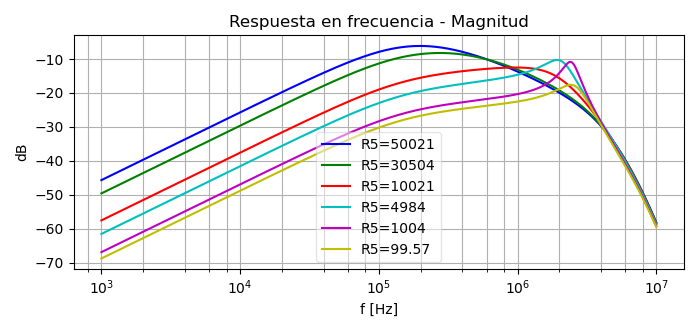
\includegraphics[width=0.47\textwidth]{../Ejercicio3-AmplificadorDeInstrumentacion/Imagenes/CM/CMVariacionR5Gain.png}\label{fig:f1}}
    \hfill
    \subfloat[Respuesta en frecuencia: diferencia de fase]{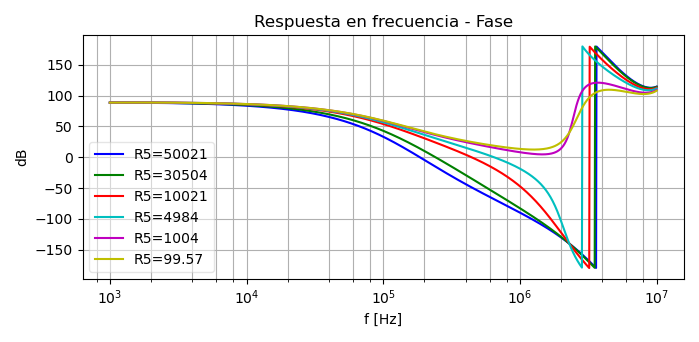
\includegraphics[width=0.4\textwidth]{../Ejercicio3-AmplificadorDeInstrumentacion/Imagenes/CM/CMVariacionR5Phase.png}\label{fig:f2}}
    \caption{Modo común: función transferencia teórica para distintos valores de $R_{5}$}
    \label{fig:R5MC}
  \end{figure}
  
  \begin{figure}[H]
    \centering
    \subfloat[Respuesta en frecuencia: ganancia]{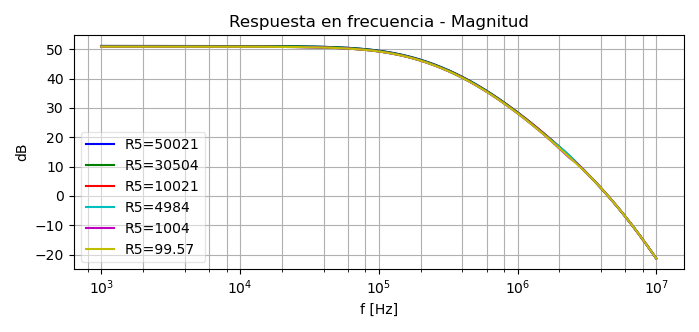
\includegraphics[width=0.47\textwidth]{../Ejercicio3-AmplificadorDeInstrumentacion/Imagenes/DM/VariacionR5Gain.png}\label{fig:f1}}
    \hfill
    \subfloat[Respuesta en frecuencia: diferencia de fase]{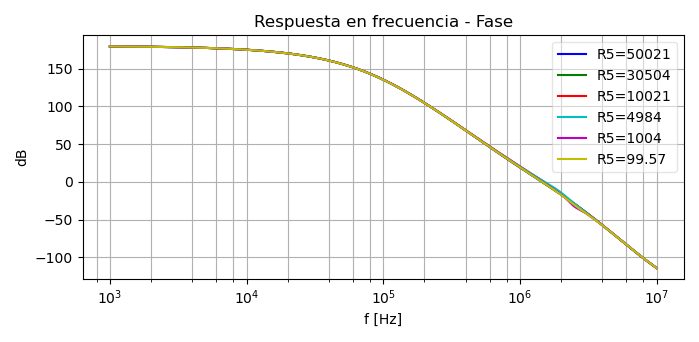
\includegraphics[width=0.4\textwidth]{../Ejercicio3-AmplificadorDeInstrumentacion/Imagenes/DM/VariacionR5Phase.png}\label{fig:f2}}
    \caption{Modo diferencial: función transferencia teórica para distintos valores de $R_{5}$}
  \end{figure}


Por otra parte, como se mencionó previamente, es importante mantener en el circuito las relaciones de resistencias para lograr un alto CMRR. No obstante, los resistores empleados cuentan con una tolerancia del $1\%$, 
pudiendo afectar el comportamiento del circuito. Para estudiar su efecto, se realizó una simulación de Monte Carlo para señales de entrada en modo común y en modo diferencial, con un valor de $R_{5}$ = $50k\Omega$.
Se presentan los resultados a continuación.

\begin{figure}[H]
    \centering
    \subfloat[Respuesta en frecuencia: ganancia]{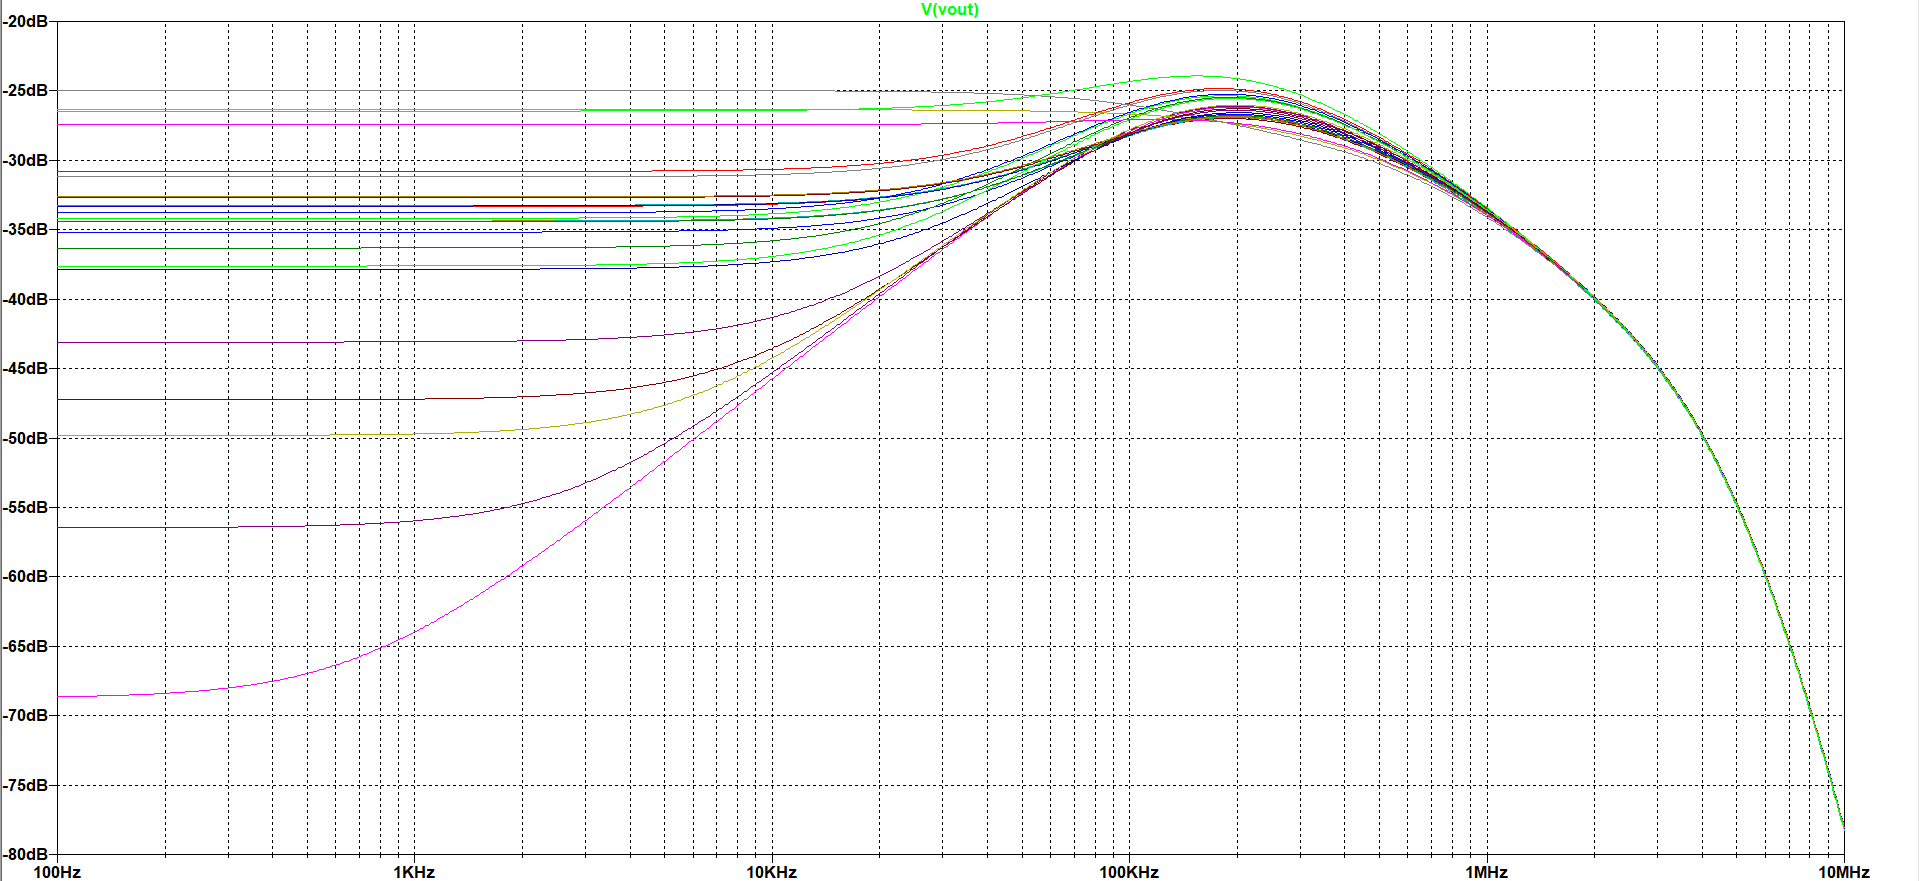
\includegraphics[width=0.47\textwidth]{../Ejercicio3-AmplificadorDeInstrumentacion/Imagenes/CM/MonteCarloGain.png}\label{fig:f1}}
    \hfill
    \subfloat[Respuesta en frecuencia: diferencia de fase]{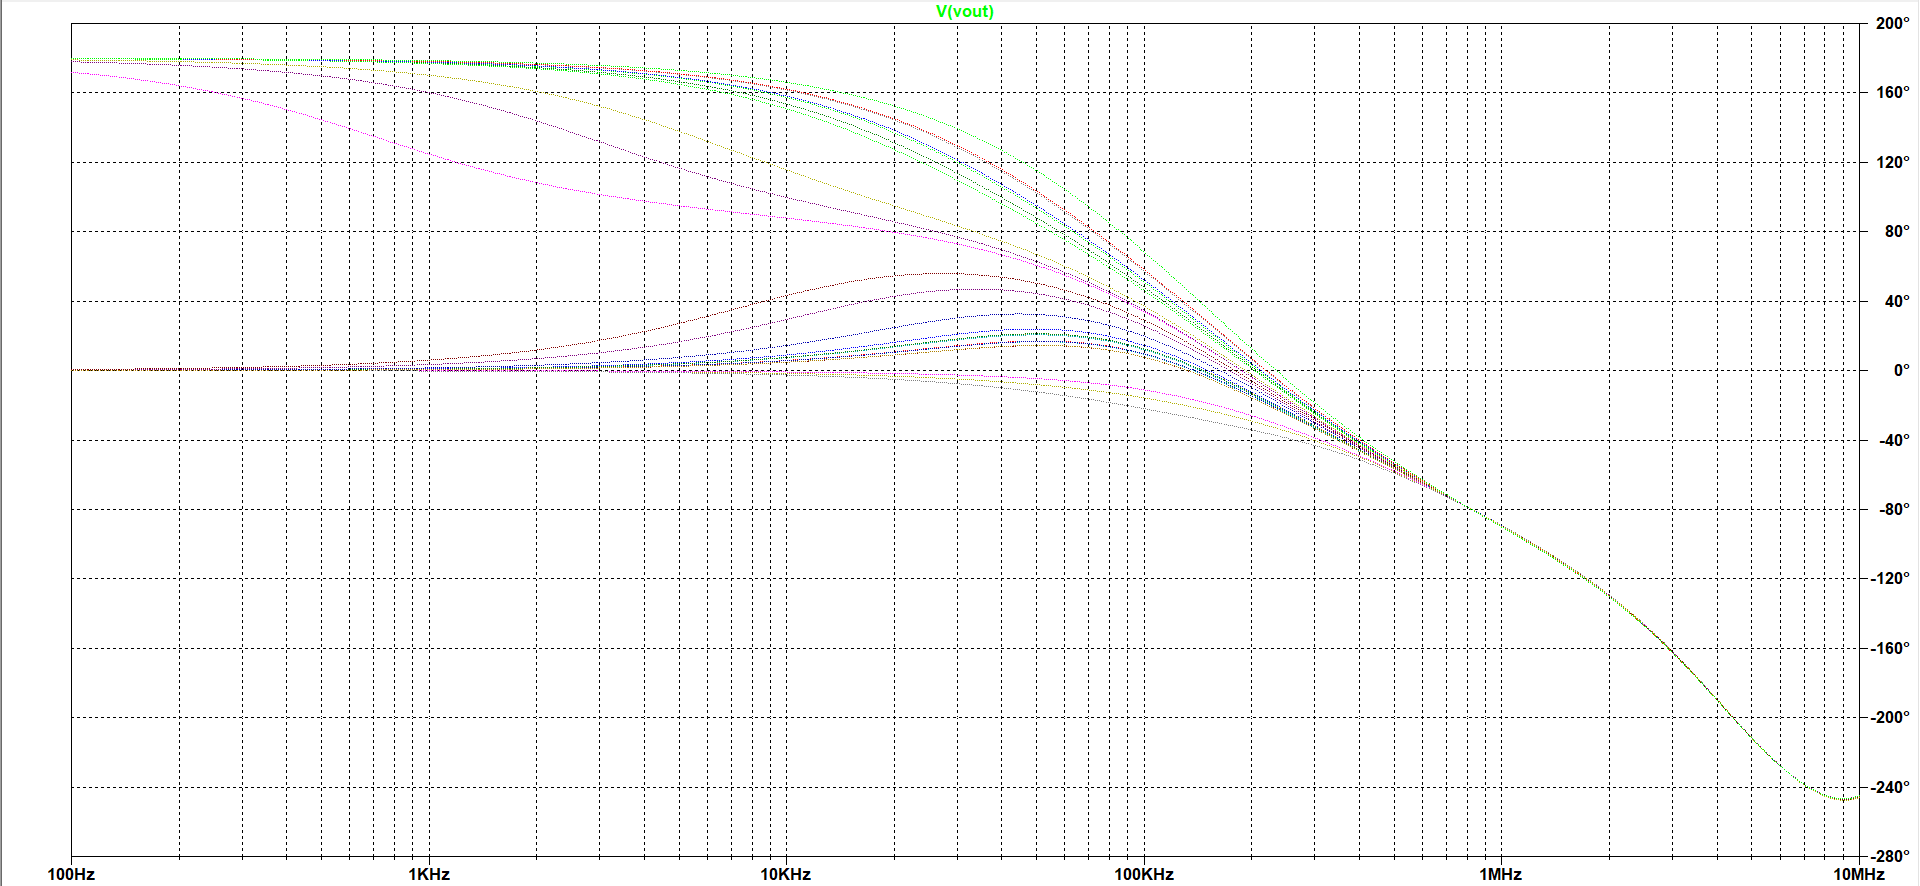
\includegraphics[width=0.47\textwidth]{../Ejercicio3-AmplificadorDeInstrumentacion/Imagenes/CM/MonteCarloPhase.png}\label{fig:f2}}
    \caption{Modo común: análisis de Monte Carlo mediante simulación con $R_{5}$ = $50k\Omega$}
  \end{figure}
  
  \begin{figure}[H]
    \centering
    \subfloat[Respuesta en frecuencia: ganancia]{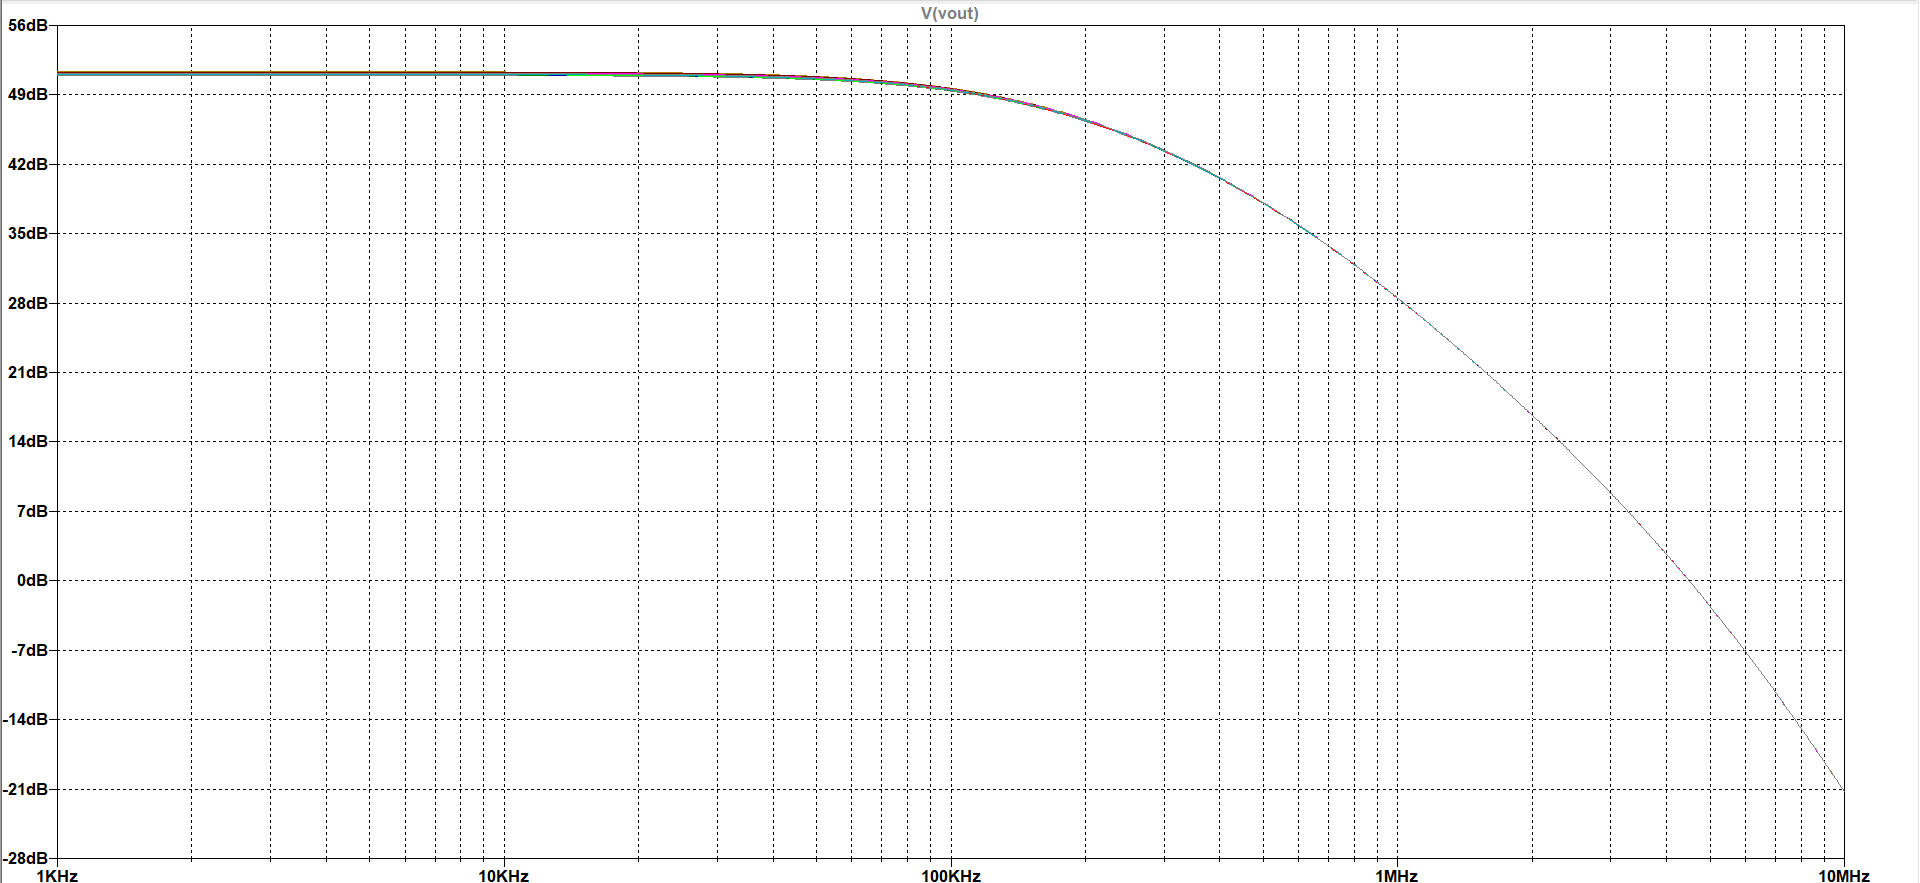
\includegraphics[width=0.47\textwidth]{../Ejercicio3-AmplificadorDeInstrumentacion/Imagenes/DM/MonteCarloGain.png}\label{fig:f1}}
    \hfill
    \subfloat[Respuesta en frecuencia: diferencia de fase]{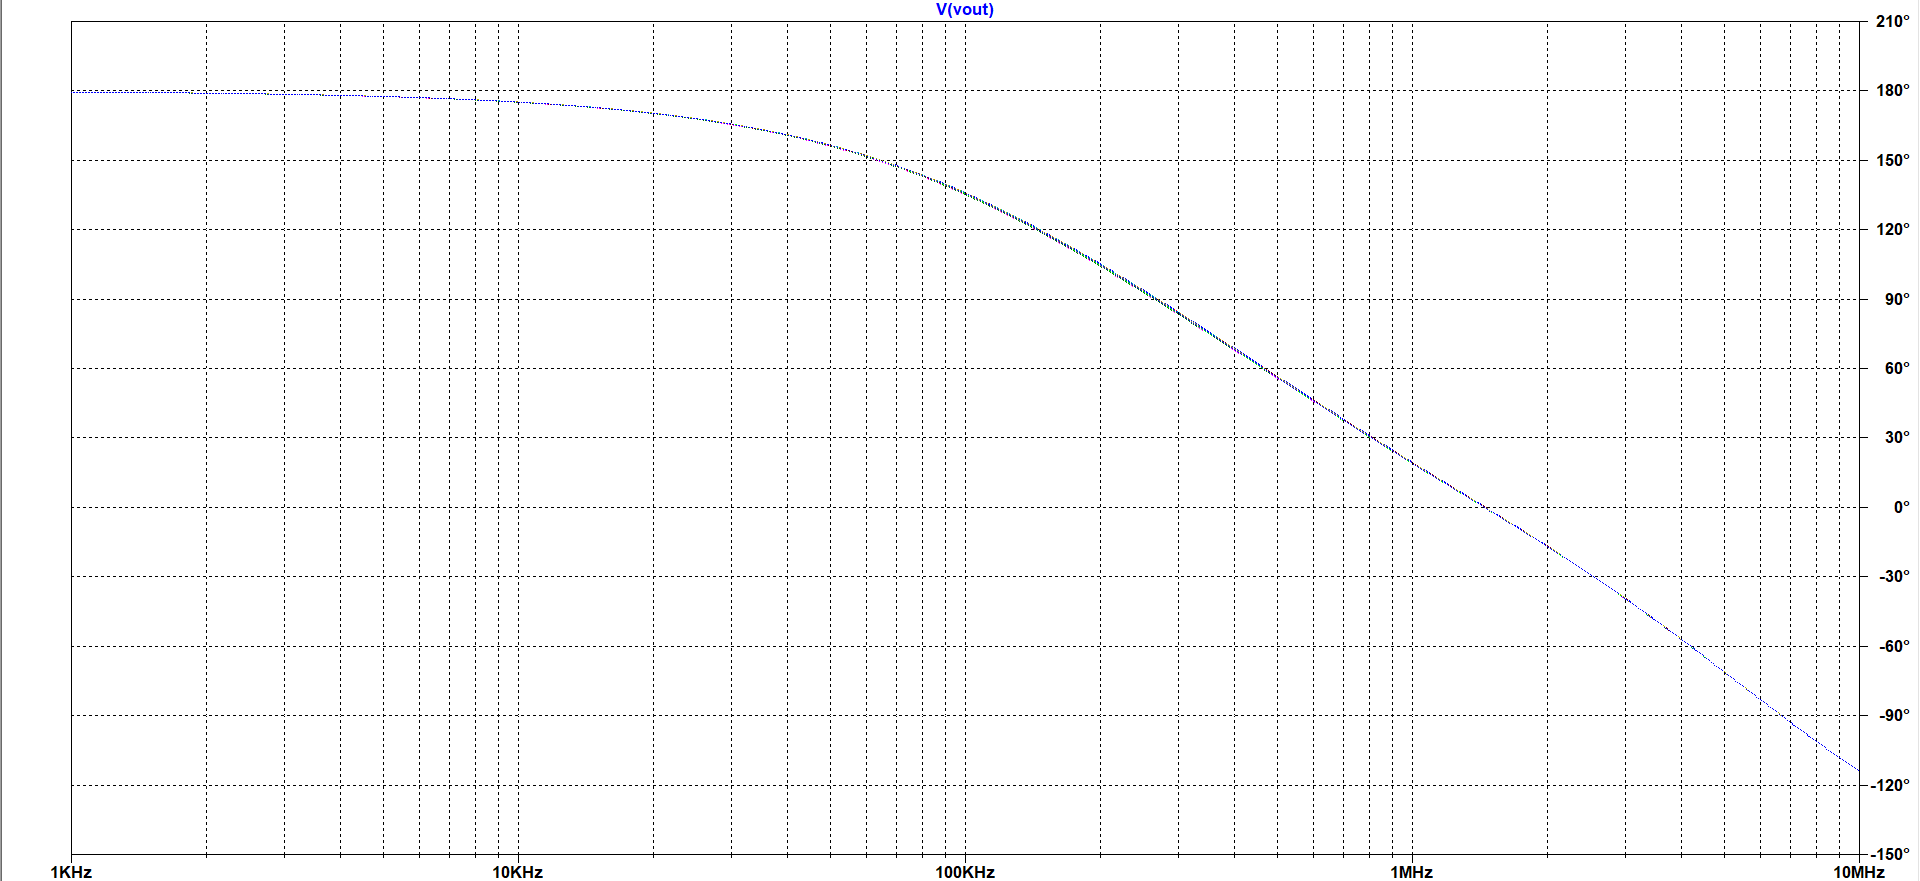
\includegraphics[width=0.47\textwidth]{../Ejercicio3-AmplificadorDeInstrumentacion/Imagenes/DM/MonteCarloPhase.png}\label{fig:f2}}
    \caption{Modo diferencial: análisis de Monte Carlo mediante simulación con $R_{5}$ = $50k\Omega$}
  \end{figure}

Se observa que nuevamente el modo diferencial no muestra grandes asimetrías aún con la variación en los valores de los resistores. En tanto, para modo común se observan mayores asimetrías respecto al caso con 
resistencias balanceadas que se presenta. En ningún caso se tiene una ganancia mayor a cero, lo cual probablemente se deba a que se realizó la simulación con un valor de $R_{5}$ que otorga estabilidad a la respuesta en frecuencia del circuito. 


Otro posible factor que afecte a la ganancia del In Amp, además de contribuir a las asimetrías de los valores medidos con respecto al modelo teórico, puede provenir de los parámetros 
de los amplificadores operacionales empleados. Para el análisis teórico se considero el valor típico de ganancia a lazo abierto
provisto por el fabricante. No obstante, se menciona un valor mínimo de $A_{ol}=25k$. Por lo tanto, resulta de interés analizar el efecto de su variación en las funciones transferencias. 

Se estudió primeramente el efecto de la variación en $A_{ol}=25k$ para el modo diferencial dado que será el modo de empleo principal del circuito. No obstante, no se encontró efecto alguno en el comportamiento
teórico de las funciones de transferencia. 

\begin{figure}[H]
    \centering
    \subfloat[Respuesta en frecuencia: ganancia]{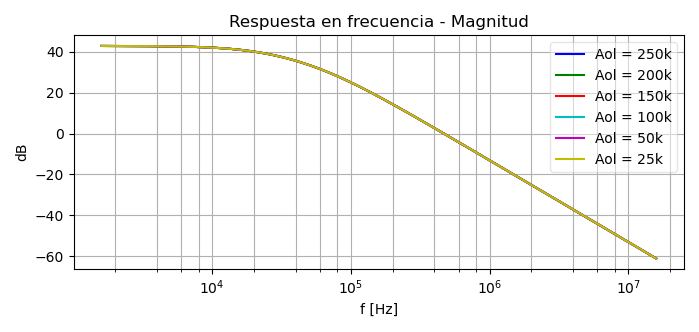
\includegraphics[width=0.47\textwidth]{../Ejercicio3-AmplificadorDeInstrumentacion/Imagenes/DM/AolvariableDMGain.png}\label{fig:f1}}
    \hfill
    \subfloat[Respuesta en frecuencia: diferencia de fase]{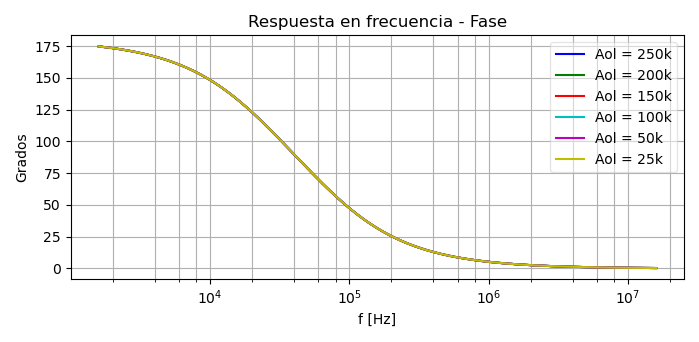
\includegraphics[width=0.47\textwidth]{../Ejercicio3-AmplificadorDeInstrumentacion/Imagenes/DM/AolvariableDMPhase.png}\label{fig:f2}}
    \caption{Modo diferencial: función transferencia teórica para distintos valores de $A_{ol}$ de los $Op$ $Amp$ en TL084.}
  \end{figure}

\subsection{Mediciones}

Se construyó el circuito en el $board$ del $Digilent$ $electronics$ $explorer$. Se emplearon dos capacitores de  de $0.1uF$ entre GND y las entradas $+V_{cc}$ y $-V_{cc}$ para reducir posibles errores por ruido dada la alta impedancia de las fuentes de alimentación. Se fijaron en el preset los valores mencionados anteriormente para $R_{5}$ para observar empíricamente su efecto sobre el circuito en ambos modos. 

Para la medición en modo común, se conectaron ambas entradas a la señal excitada por una de las salidas del generador de funciones. En cuanto al modo diferencial, se configuraron las dos salidas del generador de funciones para que funcionen de forma sincronizada, 
conectando cada uno respectivamente a una de las entradas del circuito, siendo una de las señales un poco mayor en amplitud que la otra para poder medir la amplificación de la señal diferencial a la salida. Para la medición en este modo
se debió tener especial cuidado con la saturación del circuito, por lo que se configuraron las señales de excitación con una amplitud del orden de las decenas de $mV$.

\subsubsection{Modo común}

Se obtuvo la ganancia y la diferencia de fase en respuesta a la frecuencia para los distintos valores de $R_{5}$. Se presentan los resultados superpuestos con los obtenidos de los modelos teóricos y simulados.

\begin{figure}[H]
  \centering
  \subfloat[Respuesta en frecuencia: ganancia]{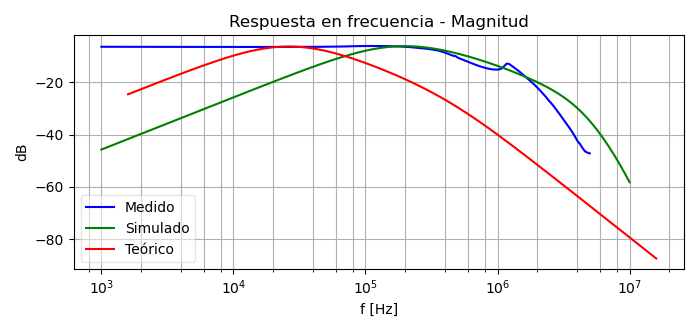
\includegraphics[width=0.47\textwidth]{../Ejercicio3-AmplificadorDeInstrumentacion/Imagenes/CM/Gain50k.png}\label{fig:f1}}
  \hfill
  \subfloat[Respuesta en frecuencia: diferencia de fase]{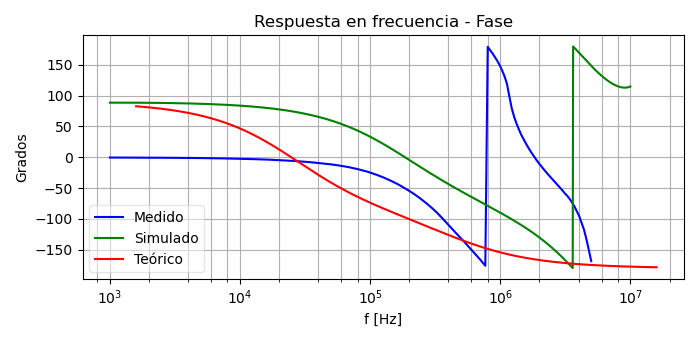
\includegraphics[width=0.47\textwidth]{../Ejercicio3-AmplificadorDeInstrumentacion/Imagenes/CM/Phase50k.png}\label{fig:f2}}
  \caption{Respuesta en frecuencia para $R_{5}$ = $50k\Omega$}
\end{figure}

\begin{figure}[H]
    \centering
    \subfloat[Respuesta en frecuencia: ganancia]{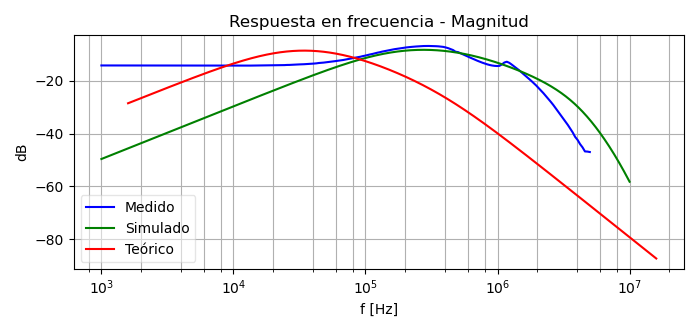
\includegraphics[width=0.47\textwidth]{../Ejercicio3-AmplificadorDeInstrumentacion/Imagenes/CM/Gain30k.png}\label{fig:f1}}
    \hfill
    \subfloat[Respuesta en frecuencia: diferencia de fase]{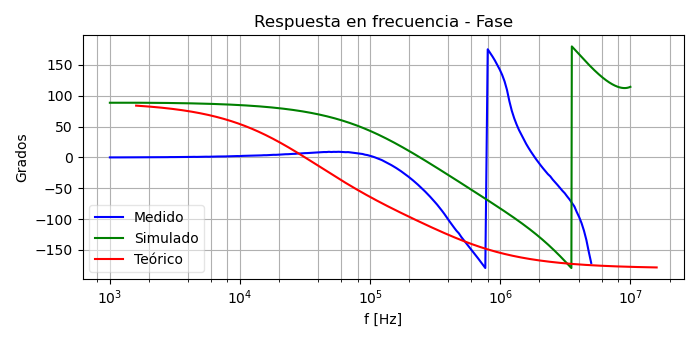
\includegraphics[width=0.47\textwidth]{../Ejercicio3-AmplificadorDeInstrumentacion/Imagenes/CM/Phase30k.png}\label{fig:f2}}
    \caption{Respuesta en frecuencia para $R_{5}$ = $30k\Omega$}
  \end{figure}

  \begin{figure}[H]
    \centering
    \subfloat[Respuesta en frecuencia: ganancia]{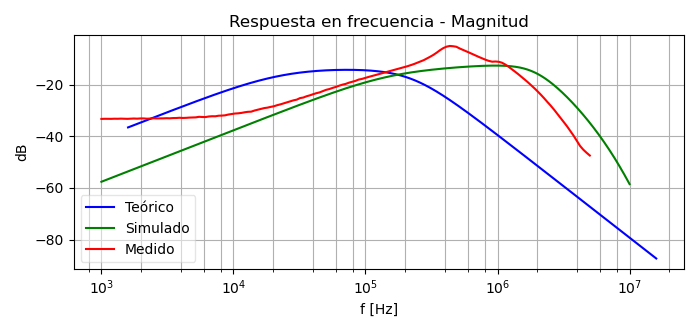
\includegraphics[width=0.47\textwidth]{../Ejercicio3-AmplificadorDeInstrumentacion/Imagenes/CM/Gain10k.png}\label{fig:f1}}
    \hfill
    \subfloat[Respuesta en frecuencia: diferencia de fase]{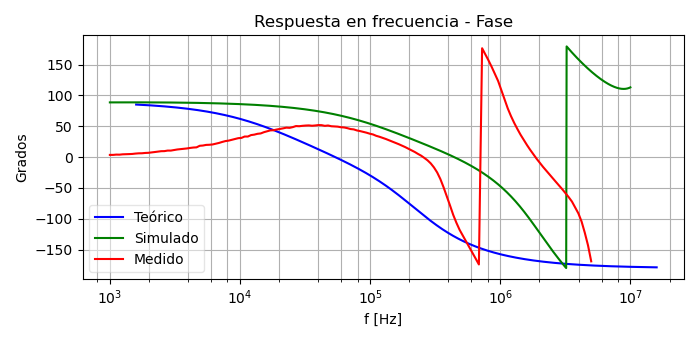
\includegraphics[width=0.47\textwidth]{../Ejercicio3-AmplificadorDeInstrumentacion/Imagenes/CM/Phase10k.png}\label{fig:f2}}
    \caption{Respuesta en frecuencia para $R_{5}$ = $10k\Omega$}
  \end{figure}

  \begin{figure}[H]
    \centering
    \subfloat[Respuesta en frecuencia: ganancia]{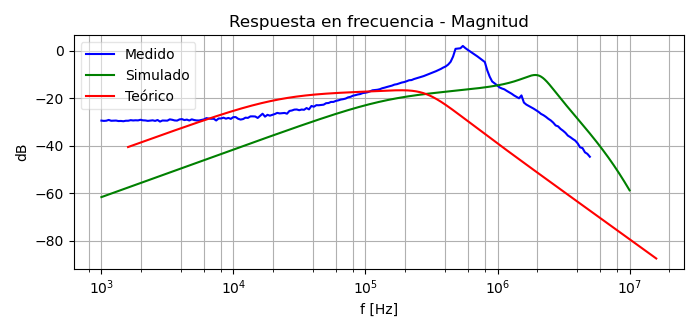
\includegraphics[width=0.47\textwidth]{../Ejercicio3-AmplificadorDeInstrumentacion/Imagenes/CM/Gain5k.png}\label{fig:f1}}
    \hfill
    \subfloat[Respuesta en frecuencia: diferencia de fase]{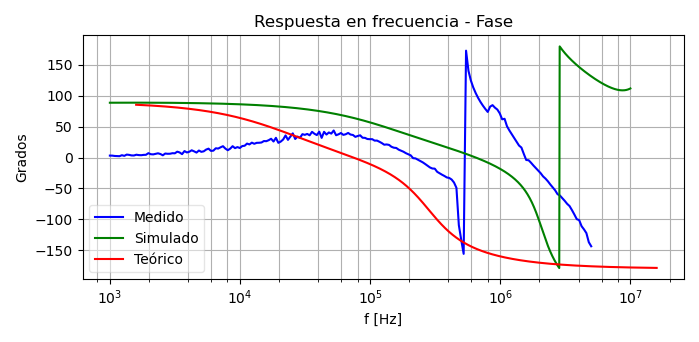
\includegraphics[width=0.47\textwidth]{../Ejercicio3-AmplificadorDeInstrumentacion/Imagenes/CM/Phase5k.png}\label{fig:f2}}
    \caption{Respuesta en frecuencia para $R_{5}$ = $5k\Omega$}
  \end{figure}

  \begin{figure}[H]
    \centering
    \subfloat[Respuesta en frecuencia: ganancia]{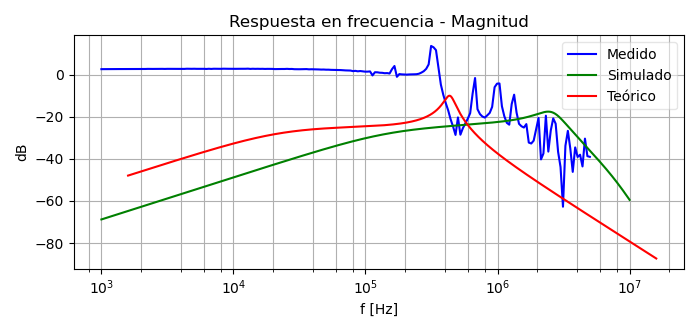
\includegraphics[width=0.47\textwidth]{../Ejercicio3-AmplificadorDeInstrumentacion/Imagenes/CM/Gain100.png}\label{fig:f1}}
    \hfill
    \subfloat[Respuesta en frecuencia: diferencia de fase]{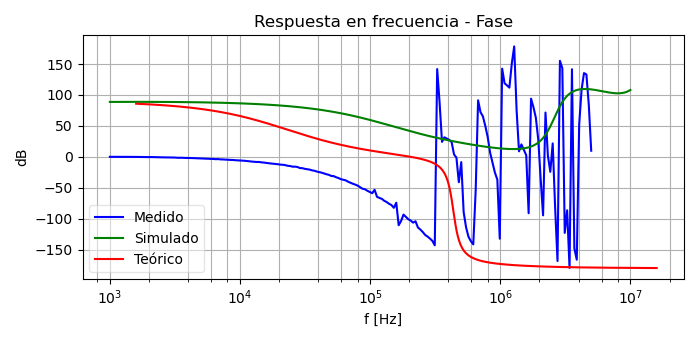
\includegraphics[width=0.47\textwidth]{../Ejercicio3-AmplificadorDeInstrumentacion/Imagenes/CM/Phase100.png}\label{fig:f2}}
    \caption{Respuesta en frecuencia para $R_{5}$ = $100\Omega$}
  \end{figure}

  En cada uno de los gráficos se presentan diferencias entre el modelo teórico y los resultados medidos y simulados, aunque se observa, especialmente en los gráficos de fase, una similitud en el comportamiento. 
  Las mayores diferencias se encuentran con bajos valores de $R_{5}$, lo cual era esperado dado la poca estabilidad del circuito en esas situaciones. Se confirma la predición teórica que para bajos valores de ese resistor se puede
  llegar a obtener una ganancia para ciertas frecuencias, lo cual no resulta conveniente para la implementación de un In Amp. 

\begin{figure}[H]
    \centering
    \subfloat[Respuesta en frecuencia: ganancia]{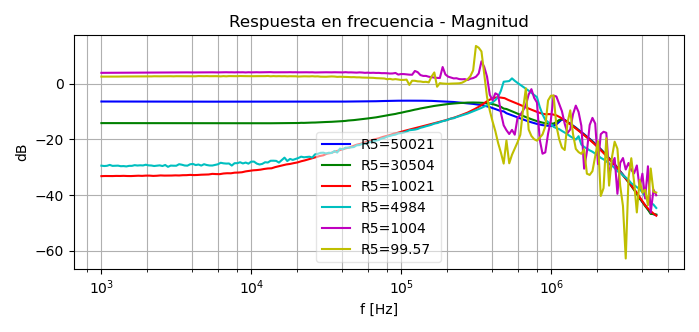
\includegraphics[width=0.47\textwidth]{../Ejercicio3-AmplificadorDeInstrumentacion/Imagenes/CM/CMAllGain.png}\label{fig:f1}}
    \hfill
    \subfloat[Respuesta en frecuencia: diferencia de fase]{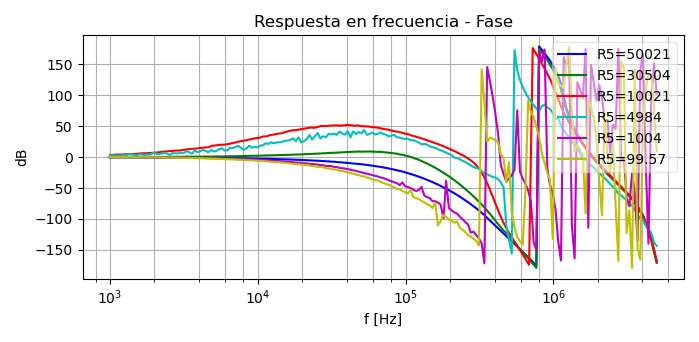
\includegraphics[width=0.47\textwidth]{../Ejercicio3-AmplificadorDeInstrumentacion/Imagenes/CM/CMAllPhase.png}\label{fig:f2}}
    \caption{Respuesta en frecuencia para $R_{5}$ = $50k\Omega$}
    \label{fig:CMsuperpuesto}
  \end{figure}



Observando en la figura \ref{fig:CMsuperpuesto} las respuestas en frecuencia de la ganancia y fase en modo común para los distintos valores superpuestas, se puede observar precisamente que bajos valores de R5 dan inestabilidad al comportamiento del circuito.


\subsubsection{Modo diferencial}

En el análisis anterior se observó que en el modo diferencial el circuito posee gran estabilidad para valores bajos y altos de $R_{5}$. Por simplificación, se estudiaron las respuestas en frecuencia para $R_{5}$ = $50k\Omega$ y $R_{5}$ = $5k\Omega$.

\begin{figure}[H]
    \centering
    \subfloat[Respuesta en frecuencia: ganancia]{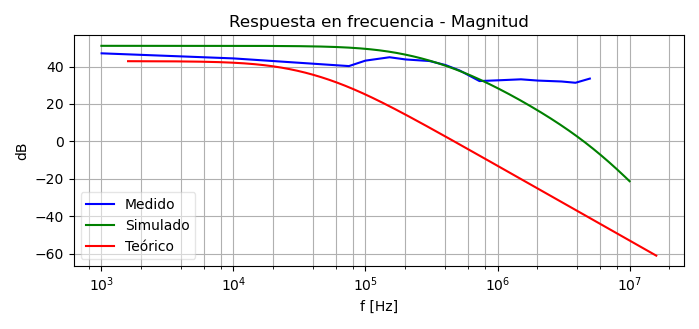
\includegraphics[width=0.47\textwidth]{../Ejercicio3-AmplificadorDeInstrumentacion/Imagenes/DM/DM50kGain.png}\label{fig:f1}}
    \hfill
    \subfloat[Respuesta en frecuencia: diferencia de fase]{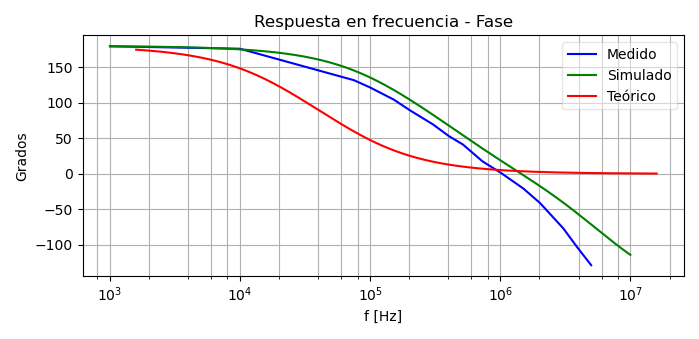
\includegraphics[width=0.47\textwidth]{../Ejercicio3-AmplificadorDeInstrumentacion/Imagenes/DM/DM50kPhase.png}\label{fig:f2}}
    \caption{Respuesta en frecuencia para $R_{5}$ = $50k\Omega$}
  \end{figure}

  \begin{figure}[H]
    \centering
    \subfloat[Respuesta en frecuencia: ganancia]{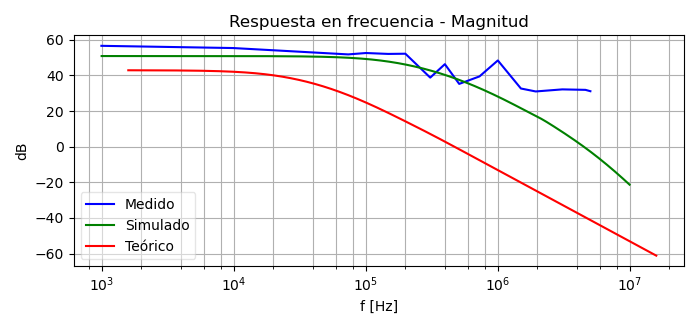
\includegraphics[width=0.47\textwidth]{../Ejercicio3-AmplificadorDeInstrumentacion/Imagenes/DM/DM5kGain.png}\label{fig:f1}}
    \hfill
    \subfloat[Respuesta en frecuencia: diferencia de fase]{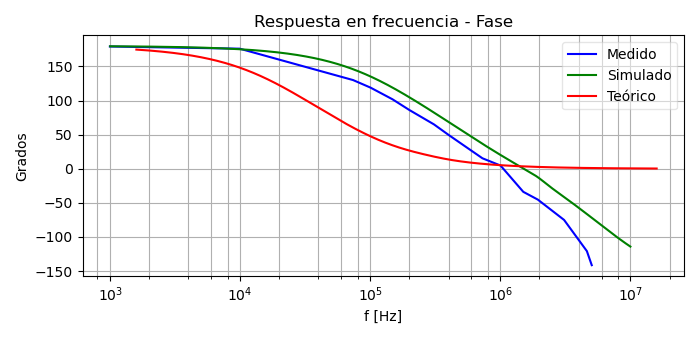
\includegraphics[width=0.47\textwidth]{../Ejercicio3-AmplificadorDeInstrumentacion/Imagenes/DM/DM5kPhase.png}\label{fig:f2}}
    \caption{Respuesta en frecuencia para $R_{5}$ = $50k\Omega$}
  \end{figure}

Se puede visualizar que se presentan diferencias entre los modelos teóricos y los resultados simulados y medidos tanto para la ganancia como para la diferencia de fase en respuesta a la frecuencia.
Donde mayores diferencias se observan es en la ganancia, mientras que en los gráficos de las fases los valores medidos se asemejan en gran grado a los simulados.

\subsection{Tensión de salida montada sobre nivel de DC}

Para que la tensión de salida del circuito aparezca montada sobre una señal continua se debe modificar la referencia del circuito. Hasta el momento, el circuito analizado posee una referencia directamente
a GND por medio de la entrada inversora del OA. Planteando una conexión a una $V_{DC}$ en dicha entrada y considerando a todos los amplificadores operacionales como ideales, tal como se vio al comienzo 
de esta sección, se tienen las siguientes relaciones en el circuito:

$$V_{o2}=V^{+}_{3}=V^{+}_{4}=V^{-}_{4} = V_{DC}$$

$$V_{o1} = \left(1+\frac{R_3}{R_4}\right)\cdot V_{1}  - \frac{R_3}{R_4}\cdot V_x$$

Teniendo por las relaciones planteadas que:

$$V_x = (1+\frac{R_6}{R_7}) \cdot V_2 - \frac{R_4}{R_3}\cdot V_{DC}$$
              
$$V_{out} = -\frac{R_{2}}{R_{1}}\cdot V_{o1} + (1+\frac{R_2}{R_1}) \cdot V_{DC} \Rightarrow V_{out} = V_{DC} - \frac{R_2}{R_1})\cdot (1+\frac{R_3}{R_4}) (V_{1}-V_{2})$$

Siendo $V_{1}=V_{2}=V_{CM}$:

$$V_{out} = V_{DC}$$

En modo diferencial se obtiene:

$$V_{out} = V_{DC} - (\frac{R_2}{R_1})\cdot (1+\frac{R_3}{R_4})\cdot V_{DM}$$

Consiguiendo de esta forma "montar" la señal de salida del In Amp sobre una tensión continua. 



